
%%%%%%%%%%%%%%%%%%%%%%% file typeinst.tex %%%%%%%%%%%%%%%%%%%%%%%%%
%
% Author: Mauricio Matamoros
% Updated: Oct 31, 2022
% Contact: mauricio@robocupathome.org
%
% This is the LaTeX source for the TDPTemplate using
% the LaTeX document class 'llncs.cls' Springer LNAI format
% used in the RoboCup Symposium submissions.
% http://www.springer.com/computer/lncs?SGWID=0-164-6-793341-0
%
% It may be used as a template for your own TDP - copy it
% to a new file with a new name and use it as the basis
% for your Team Description Paper
%
% NB: the document class 'llncs' has its own and detailed documentation, see
% ftp://ftp.springer.de/data/pubftp/pub/tex/latex/llncs/latex2e/llncsdoc.pdf
%
% Remark: Last page with specs won't be included in Camera ready TDP's.
%
% CHKTEX-FILE 8
% CHKTEX-FILE 13
%
%%%%%%%%%%%%%%%%%%%%%%%%%%%%%%%%%%%%%%%%%%%%%%%%%%%%%%%%%%%%%%%%%%%

\documentclass[runningheads,a4paper]{llncs}

% XeLaTeX support
\usepackage{ifxetex}
\ifxetex%
	\usepackage{fontspec}
	\usepackage{polyglossia}
	\setmainlanguage{english}
\else
	\usepackage[utf8]{inputenc}
	\usepackage[T1]{fontenc}
	\usepackage[english]{babel}
\fi

% Common packages
\usepackage{amsmath}
\usepackage{amssymb}
\setcounter{tocdepth}{3}
\usepackage{url}
\usepackage{float}
\usepackage{titling}
\usepackage{wrapfig}
\usepackage{booktabs}
\usepackage{csquotes}
\usepackage{fancyhdr}
\usepackage{graphicx}
\usepackage{tikz}
\usetikzlibrary{positioning}
\usepackage{lastpage}
\usepackage[all]{nowidow}
\usepackage[inline]{enumitem}
\usepackage[usenames,dvipsnames]{xcolor}

% Referencing packages
\usepackage{varioref}
\usepackage[hidelinks]{hyperref}
\usepackage[noabbrev,nameinlink]{cleveref}

\usepackage{lipsum}
\newcommand{\robospecs}{%
	\newpage%
	\pagenumbering{gobble}%
	\pagestyle{fancy}%
	\fancyhf{}%
	\chead{$|$}
	\rhead{\footnotesize\thetitle}%
	\lhead{\footnotesize\theauthor}%
	\rfoot{Robot software and hardware specification sheet}%
}

\newcommand{\BnL}[1][1em]{ \includegraphics[width=#1]{images/bnl.jpg} }



%%%%%%%%%%%%%%%%%%%%%%%%%%%%%%%%%%%%%%%%%%%%%%%%%%%%%%%%%%%%%%%%%%%%%%%%%%%%%%%%%%%%
%
% Title
%
%%%%%%%%%%%%%%%%%%%%%%%%%%%%%%%%%%%%%%%%%%%%%%%%%%%%%%%%%%%%%%%%%%%%%%%%%%%%%%%%%%%%
\title{RoBorregos Team Description Paper for\\
RoboCup@Home 2027}

\author{José Domínguez \and Alejandro González-Escamilla \and Gilberto Malagamba \and Gerardo Fregoso \and Luis Rosales \and Emil Winkler \and Camila Tite \and Fernando Hernandez-Cantu \and Luis Benvenuto \and Erick Ramírez-Cedillo \and Alberto Muñoz \and Carlos Vázquez  }

\date{
\today\endgraf\medskip
Escuela de Ingeniería y Ciencias, Tecnológico de Monterrey \\
C.P. 64849, Monterrey, N.L., Mexico\\[4pt]
\url{https://athome.roborregos.com/}\\
\url{https://github.com/RoBorregos/home2}
}

\begin{document}
\maketitle

%%%%%%%%%%%%%%%%%%%%%%%%%%%%%%%%%%%%%%%%%%%%%%%%%%%%%%%%%%%%%%%%%%%%%%%%%%%%%%%%%%%%
%
% Abstract
%
%%%%%%%%%%%%%%%%%%%%%%%%%%%%%%%%%%%%%%%%%%%%%%%%%%%%%%%%%%%%%%%%%%%%%%%%%%%%%%%%%%%%

\begin{abstract}
This paper introduces FRIDA (Friendly Robotic Interactive Domestic Assistant), a General Purpose Service Robot developed for RoboCup@Home 2027. The system employs an architecture that integrates high-level reasoning with robust low-level actuation. The four main contributions are: (1) A clutter-aware placing strategy that optimizes target poses via spatial suitability heatmaps (95\% success rate in object-placement tasks); (2) A multi-stage interpretation pipeline employing schema-aligned parsing to bridge natural language and physical execution; (3) A low-cost, open-source gripper with fractal structure soft fingertips designed for adaptive grasping; and (4) An open-source omnidirectional mecanum base whose microcontroller runs the drive kinematics and odometry fusion, enabling holonomic motion in confined domestic spaces. To support the community, the architecture, core modules and ROS 2 workspaces are open-sourced and available at: https://github.com/RoBorregos/home2.
\end{abstract}


%%%%%%%%%%%%%%%%%%%%%%%%%%%%%%%%%%%%%%%%%%%%%%%%%%%%%%%%%%%%%%%%%%%%%%%%%%%%%%%%%%%% 
\pagestyle{fancy}

% Header
\fancyhead{}
\fancyhead[R]{\small RoBorregos Team Description Paper for RoboCup@Home OPL 2027}

\section{Introduction}
RoBorregos is the representative team of Tecnológico de Monterrey, Mexico dedicated to participating in autonomous robotics competitions since 2015. Composed exclusively of undergraduate students, the team focuses on the development and dissemination of open-source robotic technologies aimed at advancing robotics research and education in Mexico. Development for the @Home league began in 2019, debuting in Mexico's @Home Beginners category in 2021 and advancing to Open Platform League in 2023 with FRIDA (Friendly Robotic Interactive Domestic Assistant). RoBorregos entered the international stage, achieving 16th place at RoboCup 2024, 6th place in 2025, and 9th place in 2026, and won 1st place at the Mexican Open 2026. Consistent with the RoboCup philosophy, RoBorregos actively contributes to the open-source community. Beyond software, we prioritize knowledge transfer: our complete source code, hardware designs, and development documentation including meeting logs and architectural decision records are publicly available. This transparency facilitates reproducibility and allows other teams to understand the rationale behind our design choices.

In addition, RoBorregos has strengthened its academic footprint through collaboration with School of Engineering and Sciences at Tecnológico de Monterrey, formalized through undergraduate research projects and peer-reviewed publications available free in our documentation webpage\footnotemark\footnotetext{\url{https://athome.roborregos.com/}}. This paper outlines the team's ongoing efforts towards a robust system capable of executing complex mobile manipulation and human-interaction tasks, such as serving guests and storing groceries, under the uncertainty of real-world environments.

\section{Research focus and interests}
The FRIDA project philosophy is focused on bridging the gap between semantic reasoning and reliable actuation in unstructured domestic environments. Driven by this goal, our research for the 2027 cycle targets specific bottlenecks in service robotics to provide reproducible contributions to the community. This year, we report significant progress in:
\begin{enumerate}

\item Context-Aware Manipulation: Fused environmental heatmaps with task constraints to generate optimal object-placing poses, ensuring collision-free trajectories in high-density clutter.

\item Reliable Neuro-Symbolic Grounding: Developed a synthetic dataset pipeline to fine-tune LLMs for reliable instruction grounding, a contribution recently published in MICAI \cite{10.1007/978-3-032-09037-9_24}.

\item Segmentation Dataset Pipeline: Upgraded semi-automatic data generation from bounding boxes to instance segmentation masks for cleaner annotations and more robust training.


\item Holonomic Mobility: Replaced the differential-drive Dashgo B1 with a custom open-source mecanum base that runs its kinematics and EKF odometry.

\end{enumerate}

\section{Robot architecture}

FRIDA operates on a distributed architecture built using ROS 2 Jazzy for communication between modules. The system is designed around a centralized task orchestrator that coordinates asynchronous independent sub-systems.

\subsection{Containerized Deployment}
The software stack is containerized using Docker to facilitate seamless multi-platform deployment on both embedded NVIDIA Jetson edge devices and standard desktop workstations. By automating environment detection and isolating complex dependencies, this architecture ensures reproducibility and lowers the barrier to entry for the open-source community, allowing researchers to deploy the system without hardware-specific configuration overhead.

\subsection{Modular Design and Standardized Communication}
The system is partitioned into four modules: Vision, HRI, Manipulation, and Navigation. By leveraging standardized ROS 2 interfaces, the underlying logic of each area is abstracted, allowing for a clear separation of concerns and a microservice-style architecture.

\section{Scientific contributions and current work}

This section details development highlights and achievements per area.

\subsection{Integration}
The system is built on a multi-layered architecture that adheres to modern software engineering standards. It employs a Hardware Abstraction Layer (HAL) to decouple high-level logic from specific device drivers, while enforcing strict module isolation to prevent cascading failures. This framework is supported by structured version control and containerized CI/CD pipelines, ensuring automated testing and reproducible deployments.

\subsubsection{Software Architecture.} Task-specific deterministic Finite State Machines (FSM) orchestrate the high-level logic; sub-task coordinators provide abstracted functions for calling nodes at module-level; at the lowest level, modules interact with the hardware and execute primitive actions.

\subsubsection{Task Planning.} The use of FSMs facilitates logic-driven translation of complex tasks into concrete and robust robotic behaviors. It allows the incorporation of dynamic planning and fault tolerance which enables: receiving feedback for grounding the robot's actions, ease of testing by mocking responses from certain modules, and the incorporation of retry mechanisms in case sub-task functions fail, along with fallback policies involving asking humans for help (Deus ex machina).

\subsection{Object Manipulation}

The manipulation pipeline integrates perception, planning, and a custom end-effector to perform robust picking, placing, and pouring tasks.

\subsubsection{Motion Planning Strategy.} 
RRTConnect \cite{kuffner2000rrt} is employed to generate collision-free trajectories, applying path constraints in the configuration space to maintain end-effector orientation (e.g., to prevent spillage). 
To minimize latency, the planning scene is abstracted: RANSAC \cite{martinez2022ransac} segments the table plane and object clusters, which are then approximated as primitive boxes and bounding spheres. This geometric simplification reduces collision checking from expensive mesh-to-mesh queries to efficient algebraic primitive tests.


\subsubsection{Picking.} Target objects are isolated by fusing 2D detections with 3D point clouds using multi-threaded parallel filtering and variable-resolution downsampling to maximize CPU throughput. Grasp Pose Detection (GPD) \cite{ten2017grasp} generates candidate poses within this simplified scene, which are executed by the motion planner.


\subsubsection{Placing \& Pouring.} Both tasks require strict constraint handling. For placing, a suitability costmap is generated by fusing a base Gaussian distribution (favoring free space) with a constraint heatmap created by projecting Gaussian fields along relative vectors (e.g., for "place in front of X") (Fig. \ref{fig: heatmap}).
Similarly, for pouring, PCL \cite{rusu20113d} analyzes the container’s rim height to define a trajectory that strictly respects the orientation constraints defined in the motion planning phase.

\begin{figure}[H]
    \centering
    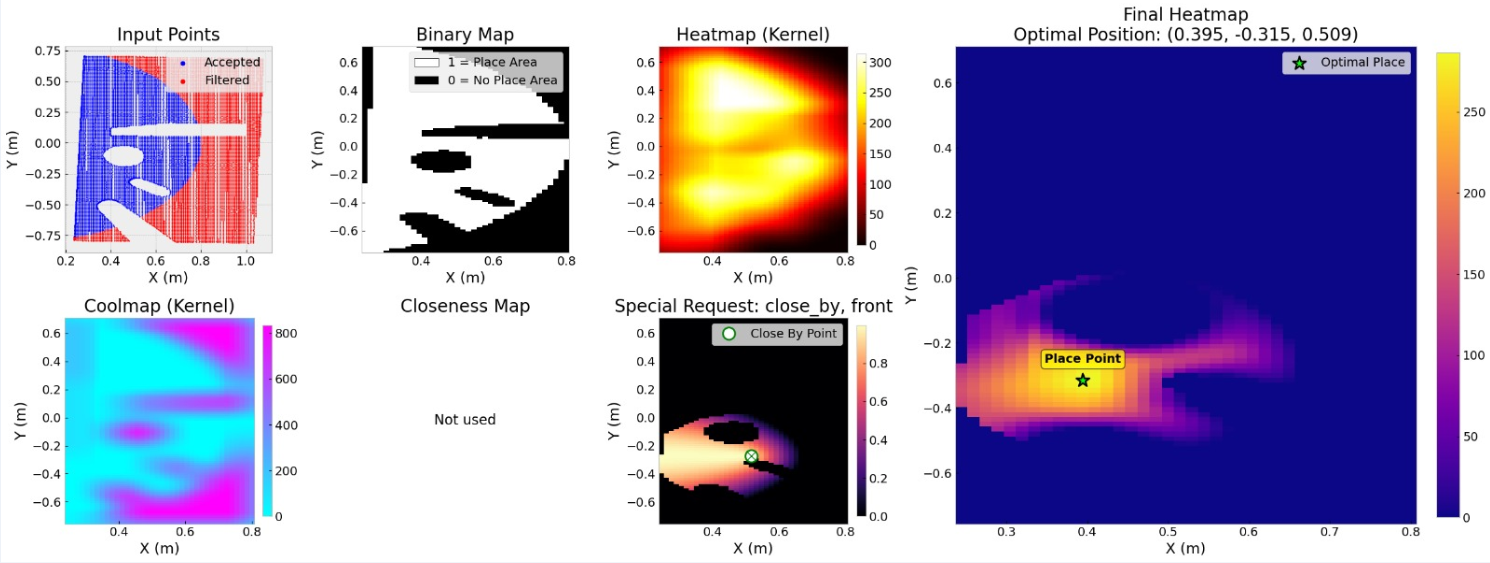
\includegraphics[width=0.8\textwidth]{TDPTemplate-master/images/HeatMaps.png}
    \caption{Heatmaps for an "in front" of placement request.}
    \label{fig: heatmap}
\end{figure}

\subsubsection{Experimental Validation.} Robustness was evaluated through 40 trials (20 picking, 20 placing), with randomized configurations of household objects (e.g., an apple surrounded by diverse objects). Results are shown in Table \ref{tab:manipulation_results}.

\textit{Picking Reliability.} Failures stemmed primarily from motion planning constraints in high density scenarios and dynamic interactions with spherical objects (e.g., orange rolling upon contact).

\textit{Placing Reliability.} Heatmap logic effectively directed placement to free space. The single failure resulted from a minor collision with an adjacent object during retraction, though the placed object remained stable.

\begin{table}[h]
\centering
\caption{Manipulation Success Rates.}
\label{tab:manipulation_results}
\begin{tabular}{lccc} 
\toprule
\textbf{Task Phase} & \textbf{Successes} & \textbf{Attempts} & \textbf{Success Rate (\%)} \\ 
\midrule
Object Picking & 16 & 20 & 80\% \\ 
Object Placing & 19 & 20 & 95\% \\ 
\bottomrule
\end{tabular}
\end{table}

\subsubsection{Custom Gripper.} A low-cost, easy-to-manufacture, open-source\footnotemark\footnotetext{\url{https://grabcad.com/library/robotic-gripper-34}}, custom parallel gripper, powered by a rack-and-pinion mechanism and a high-torque servo, secures objects up to 1 kg. Its novelty lies in fingers incorporating fractal-structured silicone covers \cite{cuan} and soft inner materials, enhancing deformation and adaptability to complex geometries (see Fig. \ref{fig:gripperGraspingPositions}).

\begin{figure}[H]
    \centering
    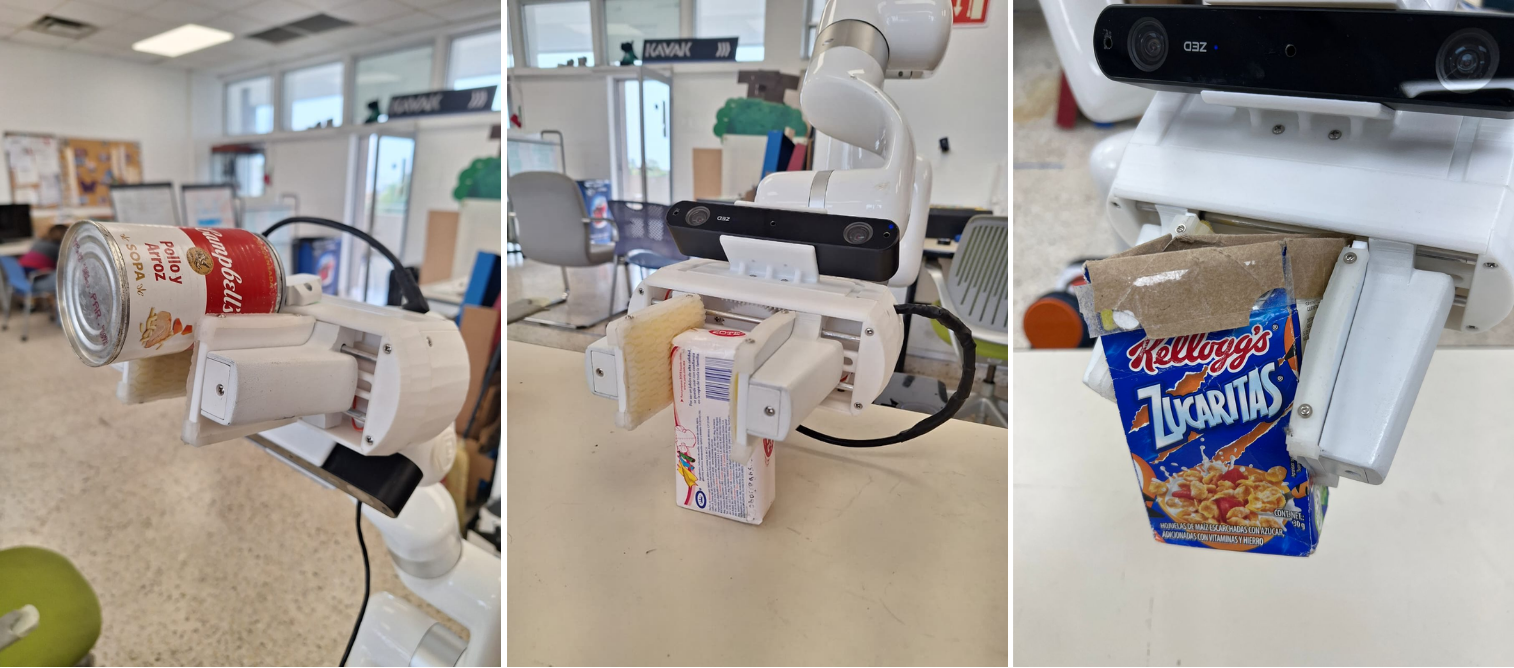
\includegraphics[width=0.7\textwidth]{TDPTemplate-master/images/gripperGraspingPositions.png}
    \caption{Gripper grasps from different positions.}
    \label{fig:gripperGraspingPositions}
\end{figure}

\subsection{Computer Vision}

\subsubsection{Face Recognition.}


\subsubsection{Person Tracking and Re-identification.}
YOLOv8n with ByteTrack~\cite{bytetrack} tracks the person being followed frame by frame, while a Re-ID module recovers the identity after occlusions. The Re ID network is a Swin Transformer trained on Market1501 with the Person ReID baseline~\cite{joint_reid}, chosen for its discriminative embeddings. While the target is visible, its embeddings are stored at a limited rate in a rolling gallery of up to 128 vectors, which captures appearance changes as the person moves. When the track is lost, each visible person is compared against the gallery by cosine similarity, and the best match. Re ID runs asynchronously in FP16 on the GPU, keeping the tracking loop fast.

\subsubsection{Pose and Gesture Recognition.}
MediaPipe~\cite{mediapipe} extracts skeletal landmarks for gesture inference. A Vision Language Model (VLM)~\cite{moondream} is queried on cropped person images to infer pose and clothing attributes.

\subsubsection{Object Detection.}
A self-hosted web pipeline\footnote{\url{https://github.com/RoBorregos/home-pipelines}} turns a 20-second phone video per object into a trained detector. GroundingDINO~\cite{grounding_dino} localizes each object from its class name and SAM3~\cite{sam3} refines its mask, producing clean crops that are reviewed in the browser and stored in a shared repository reused across parallel runs. Crops are composited onto real backgrounds to generate labeled, augmented datasets, and YOLO is trained on two NVIDIA A6000 GPUs. At RoboCup 2026, a single member operating the pipeline from a phone recorded, trained, and deployed a 30-class competition detector in 5 hours, reaching a mean Average Precision (mAP) of 97.76\% over IoU 0.5--0.95 on the validation set.

\subsubsection{Few-shot Object Recognition (Embedding Gallery).}
For objects announced shortly before a test, we added a path that needs only 15/20 photos per class and no retraining. YOLOE~\cite{yoloe} proposes class agnostic boxes, DINOv2~\cite{dinov2} embeds each crop, and the crop is compared by cosine similarity against the gallery embeddings of each class. It is less precise than our main supervised detector, but still performs well, 92.2\% proposal recall and 80.6\% gated recall@1.

\subsection{Human-Robot Interaction (HRI)}

\subsubsection{Speech.} The main communication interface with users is through audio. Speech To Text (STT) is performed via an adaptation of the WhisperLive~\cite{whisperlive} implementation using a faster-whisper backend. This enables interpreting a stream of output text and providing feedback or a reaction whilst the user is speaking. Text To Speech (TTS) is also performed live, leveraging the open-weight, fast, and efficient model Kokoro-82M~\cite{hexgrad_2025}. Together, they provide a seamless and time-sensitive user experience. These modules are containerized outside the ROS environment by leveraging lightweight and high-performance gRPC communication contributing to the microservice style architecture.

\subsubsection{Display.} A secondary  user interface is displayed on a screen in the robot's base. It provides insights into FRIDA's processes, allowing users to better understand how and when to interact with it. Some examples include displaying icons prompting users to speak, live STT transcriptions, TTS dialog, detected keywords, vision detections with bounding boxes, and voice activity detection levels.  The web UI is implemented in Next.js which connects to the WebSockets provided by rosbridge.

\subsubsection{Command Interpreter.} This pipeline translates natural language into robot-executable tasks. The process is handled by a fine-tuned Llama 3.1 8B model trained on a synthetically generated dataset. It is locally hosted via the Ollama framework on an Nvidia Orin AGX which provides sufficient VRAM.

The dataset is generated through a structured pipeline that begins with a set of predefined command templates which are populated with random variable entities (e.g., names, locations, and objects) and follow-up instructions. Entries are then generated by outputting a paraphrased natural-language instruction and a corresponding structured action plan composed of predefined primitive actions. During inference, the BAML framework parses the LLM's output into a strict JSON format avoiding action-level hallucinations, and a RAG system grounds commands ensuring entities are present in the current context.

    
This open source research was published by RoBorregos winning 2nd Best Student Paper at the 24th Mexican International Conference on Artificial Intelligence~\cite{10.1007/978-3-032-09037-9_24}.


\subsection{Navigation}

\subsubsection{Stack overview.}
FRIDA's navigation is built on the ROS~2 Navigation Stack
Nav2~\cite{macenski2020marathon2} and runs inside a single Docker container.
SLAM Toolbox~\cite{macenski2021slamtoolbox} builds 2D maps of the arena from
the combined scan of the two RPLIDAR~C1 sensors, using graph-based SLAM with
loop closure, and is then run in localization mode on the saved map. Wheel and
inertial odometry are fused by an EKF on the base controller
and provide the motion estimate for localization.
\subsubsection{Planning and Control.}
Global paths are computed with Nav2's NavFn planner using A* search, while a
Model Predictive Path Integral (MPPI) controller~\cite{williams2016mppi}
handles local trajectory tracking. The controller uses a holonomic motion
model, allowing FRIDA to move laterally when approaching furniture or
navigating narrow passages. The local and global costmaps combine the lidar
scan with a spatio-temporal voxel layer built from the RGB-D point cloud,
which captures obstacles outside the lidar plane and lets stale voxels decay
over time, so that phantom obstacles are cleared even while the robot is
stationary.
\subsubsection{Behavior Tree and Supervision.}
Nav2's behavior tree coordinates path planning, goal execution and recovery
behaviors. A custom supervisor monitors the sensor streams and transforms
required by SLAM and Nav2. If any of them becomes unavailable, it pauses both
components and resumes them once the required data is restored. The supervisor
also provides the task manager with a reduced set of navigation services.


\section{Conclusions and future work}

The contributions to the @Home league include general-purpose modules for perception, manipulation, navigation, and HRI, integrated into a cohesive layered architecture. Participation in RoboCup 2026 demonstrated FRIDA’s ability to perform core @Home tasks such as speech-based interaction, person and object recognition, autonomous navigation, and object picking and placing in cluttered environments. Current limitations include two-handed tasks such as lifting a laundry basket or folding clothes, imposed by a single arm with limited reach and an on-arm camera, motivating future work on a bimanual platform, Vision-Language-Action (VLA) models, imitation learning, and a static camera for real-time feedback.


\bibliographystyle{unsrt}
\bibliography{bibliography}


\newpage

\section*{Annex}

%CHKTEX-FILE 46

\subsection*{FRIDA Hardware Description}
\label{sec:annex-OPL}
% In this section briefly describe the software and hardware of the robot

\setlength\intextsep{0pt}
\begin{wrapfigure}[10]{h}{0.33\textwidth}
	\centering
	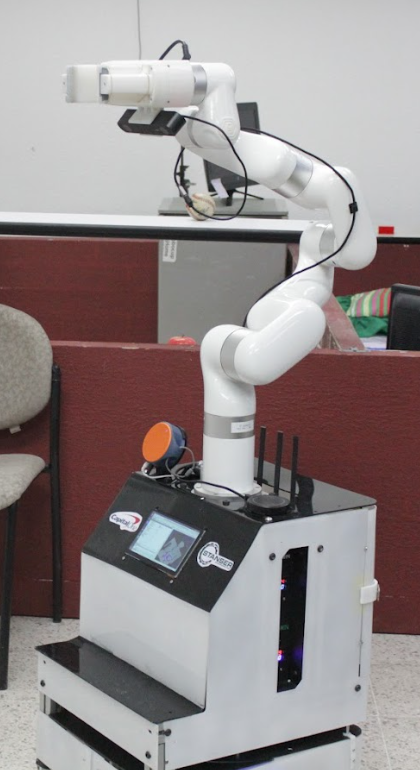
\includegraphics[width=0.3\textwidth]{TDPTemplate-master/images/frida.png}
	\caption{FRIDA}%
	\label{fig:frida}
\end{wrapfigure}

\begin{itemize}
	\item Base: A modified EAI Dashgo B1 differential drive robot was used for mobility purposes and motors with encoders for odometry purposes.
	\item Computers: NVIDIA Jetson AGX Orin 64GB.
	\item Batteries: A total of three 24v li-ion batteries are used, one for the xArm, Jetson Orin and Dashgo.
	\item Manipulator: xArm 6.
    \item Gripper: 2 finger parallel custom 3D printed gripper with force resistive sensors on each finger and an IR sensor for detecting objects in front of it. It uses an ESP32 as the microcontroller.
	\item Vision: Stereolabs ZED2 camera attached to the EOF of the xArm that runs the vision tasks and transmits data through a USB cable to the Jetson Orin.
        \item HRI: Seed Studio ReSpeaker Microphone array, Logitech X100 Wireless Portable Speaker, and a HDMI LCD touch screen 7" display.
        \item Navigation: RP Lidar A1.
        \item Base cover: Custom acrylic manufactured structure to protect and secure the interior electronics and components.
	\item Robot dimensions: Height 180 cm (fully extended), base footprint 50 cm $\times$ 42 cm
	\item Robot weight: 40 kg.
\end{itemize}

\subsection*{FRIDA Software Description}

\begin{itemize}
	\item Platform: ROS 2, Jazzy distribution.
    \item Integration: Docker
	\item Navigation: ROS 2 Navigation Stack, RTAB-Map
	\item Person analysis: Torch, InsightFace, YOLO11-pose, MediaPipe, ByteTrack, Moondream2
	\item Speech recognition: WhisperLive with faster-whisper
    \item Keyword spotting: Open Wake Word
	\item Text processing: Llama 3.2, sentence-transformers/ all-MiniLM-L6-v2
    \item Text To Speech: Kokoro-82M
	\item Object detection: GroundingDINO, SAM 3, YOLO11, YOLOE, DINOv2
    \item Manipulation planning: MoveIt 2, GPD
    \item Point cloud processing: PCL, RANSAC
\end{itemize}


%CHKTEX-FILE 46
%\section*{Annex}
%\label{sec:appendix-OPL}
%\setcounter{section}{0}

% \subsection*{Appendix 1}
% \begin{figure}[H]
%     \centering
%     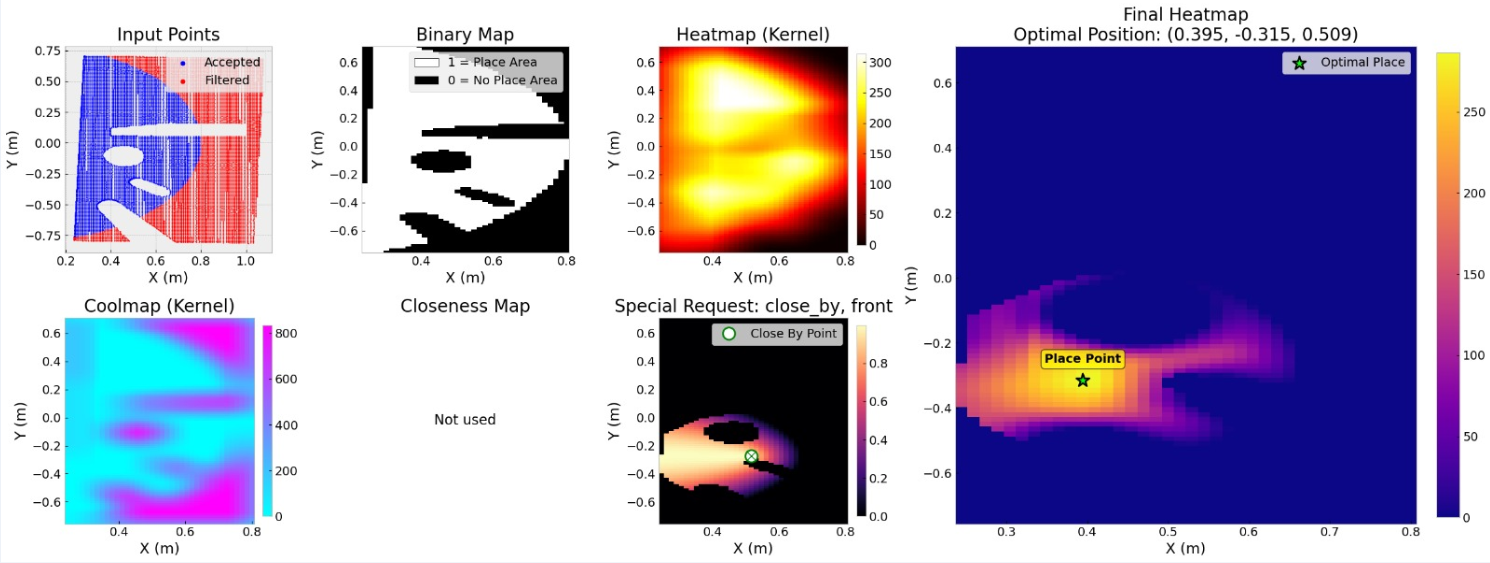
\includegraphics[width=1\textwidth]{TDPTemplate-master/images/HeatMaps.png}
%     \caption{Heatmaps generated to attend a request to place an object in front of another one.}
%     \label{fig: heatmap}
% \end{figure}

% \subsection{Pipeline}
% \begin{figure}[H]
%     \centering
%     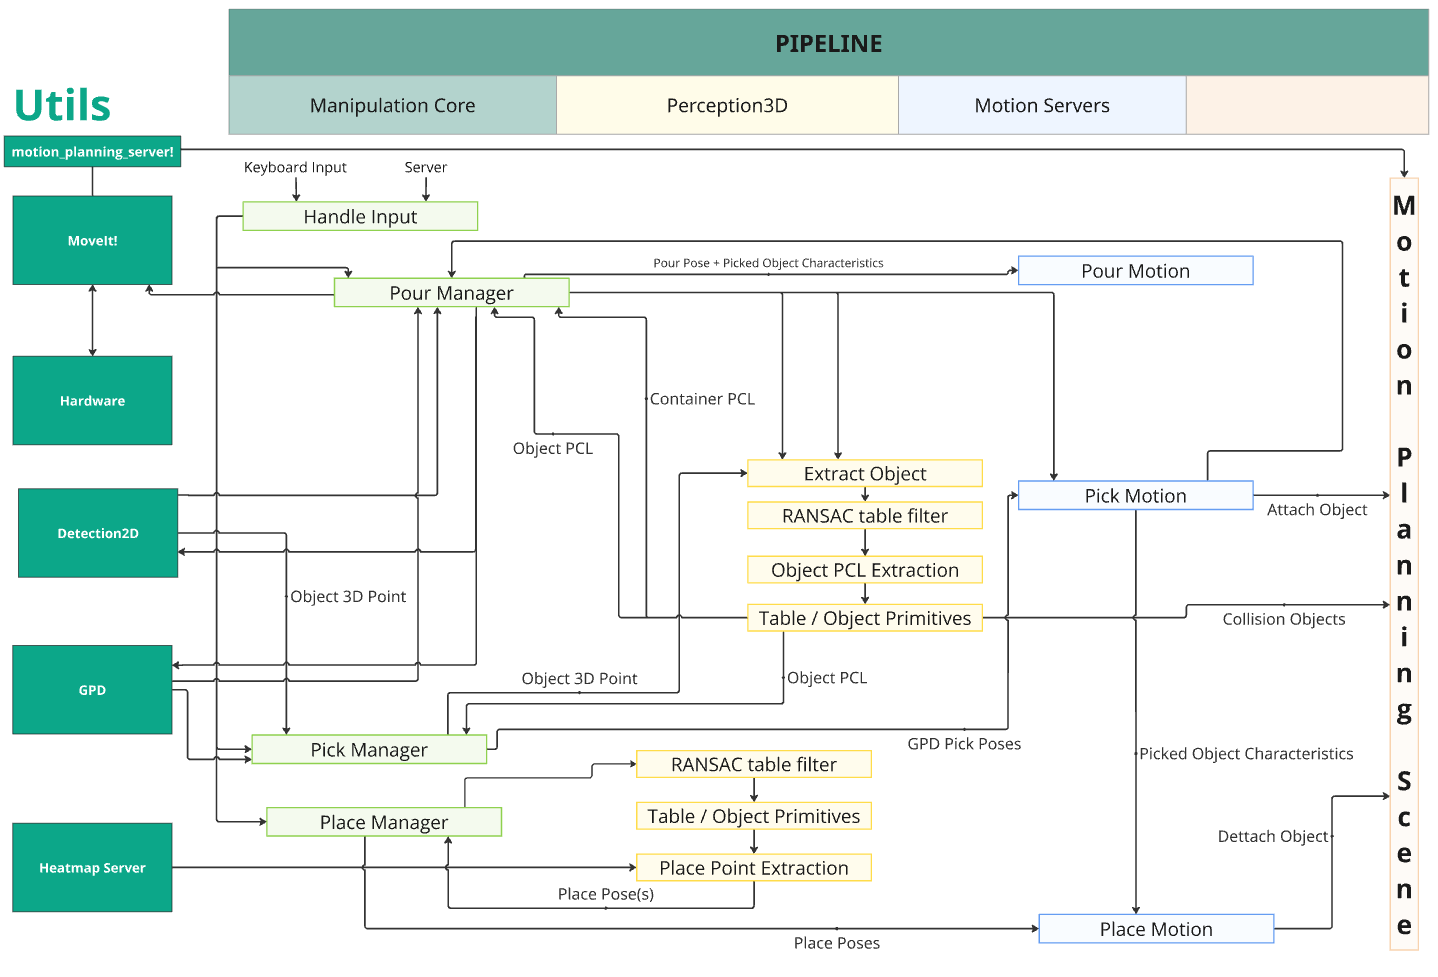
\includegraphics[width=.7\textwidth]{TDPTemplate-master/images/ManpulationPipeline.png}
%     \caption{Manipulation Pipeline with Pick, place and pour in Ros2}
%     \label{fig: manipPipeline}
% \end{figure}

% \subsection*{Appendix 2}
% \begin{figure}[H]
%     \centering
%     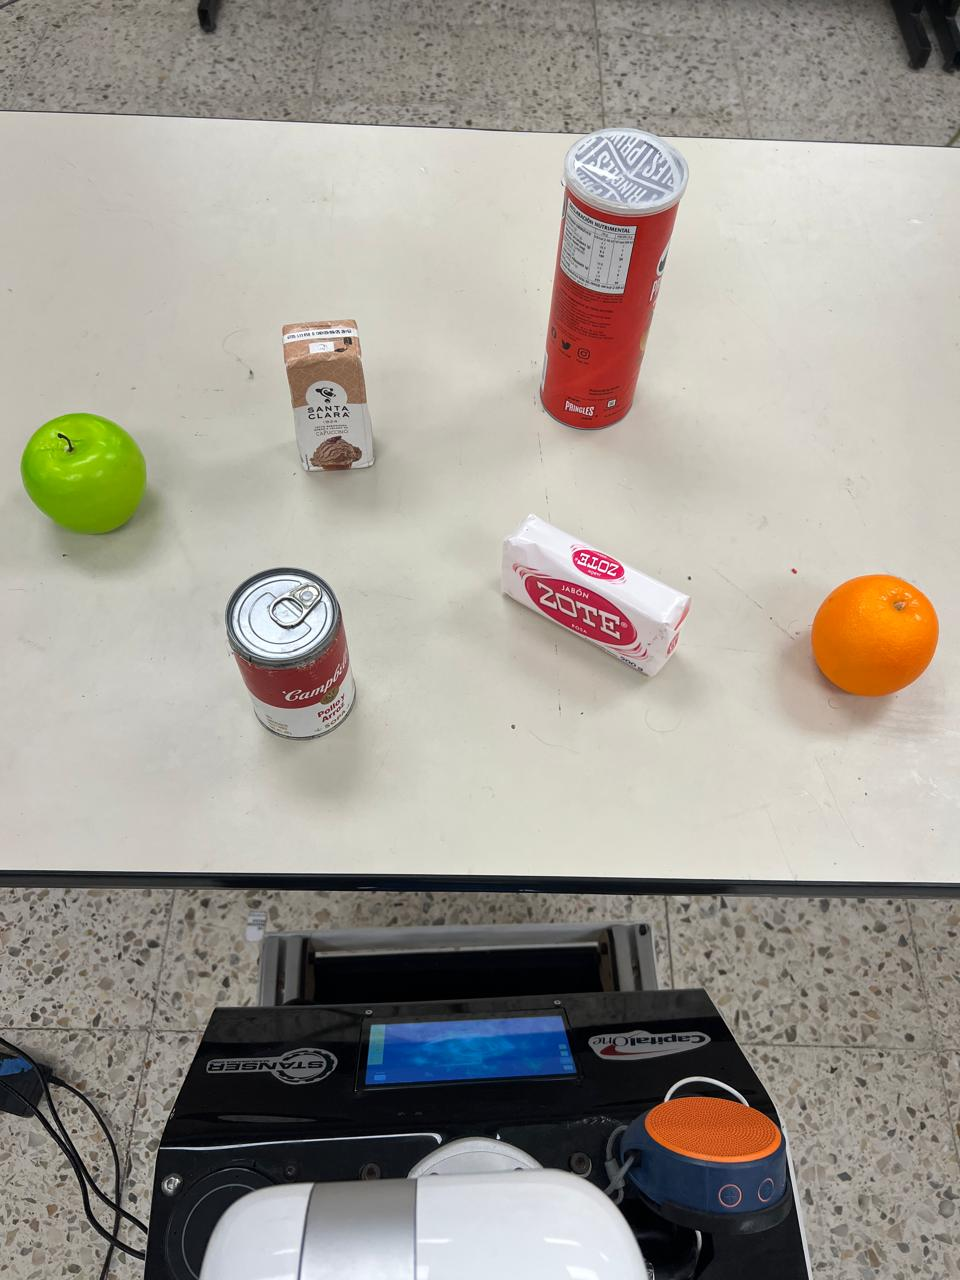
\includegraphics[width=0.55\textwidth]{TDPTemplate-master/images/pick_placeEnv.jpeg}
%     \caption{Experimental setup for Pick \& Place tasks.}
%     \label{fig:pick_place_env}
% \end{figure}

% \subsection*{Appendix 3}
% \begin{figure}[H]
%     \centering
%     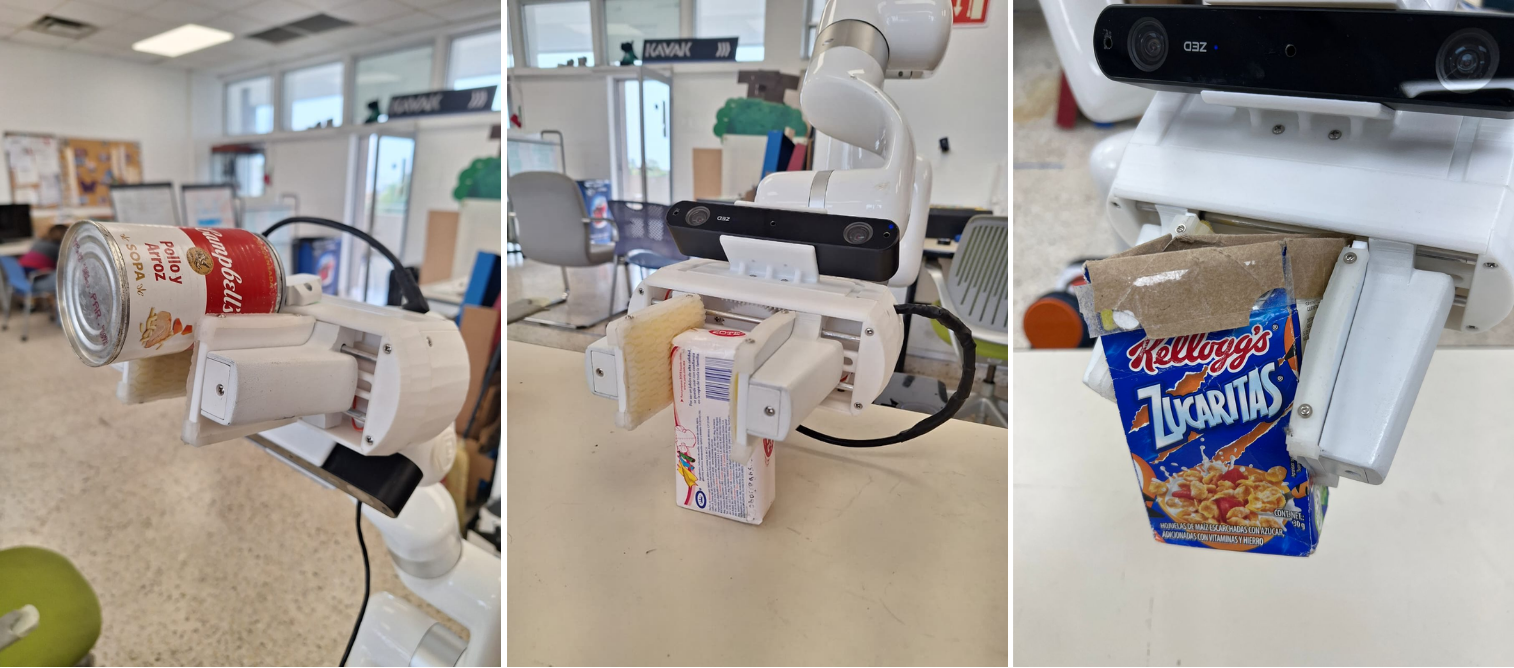
\includegraphics[width=0.95\textwidth]{TDPTemplate-master/images/gripperGraspingPositions.png}
%     \caption{Gripper grasps from different positions.}
%     \label{fig:gripperGraspingPositions}
% \end{figure}

% \section{Computer Vision}
% \subsection{Overview of the Robot’s Computer Vision Pipeline}
% \begin{figure}[H]
%     \centering
%     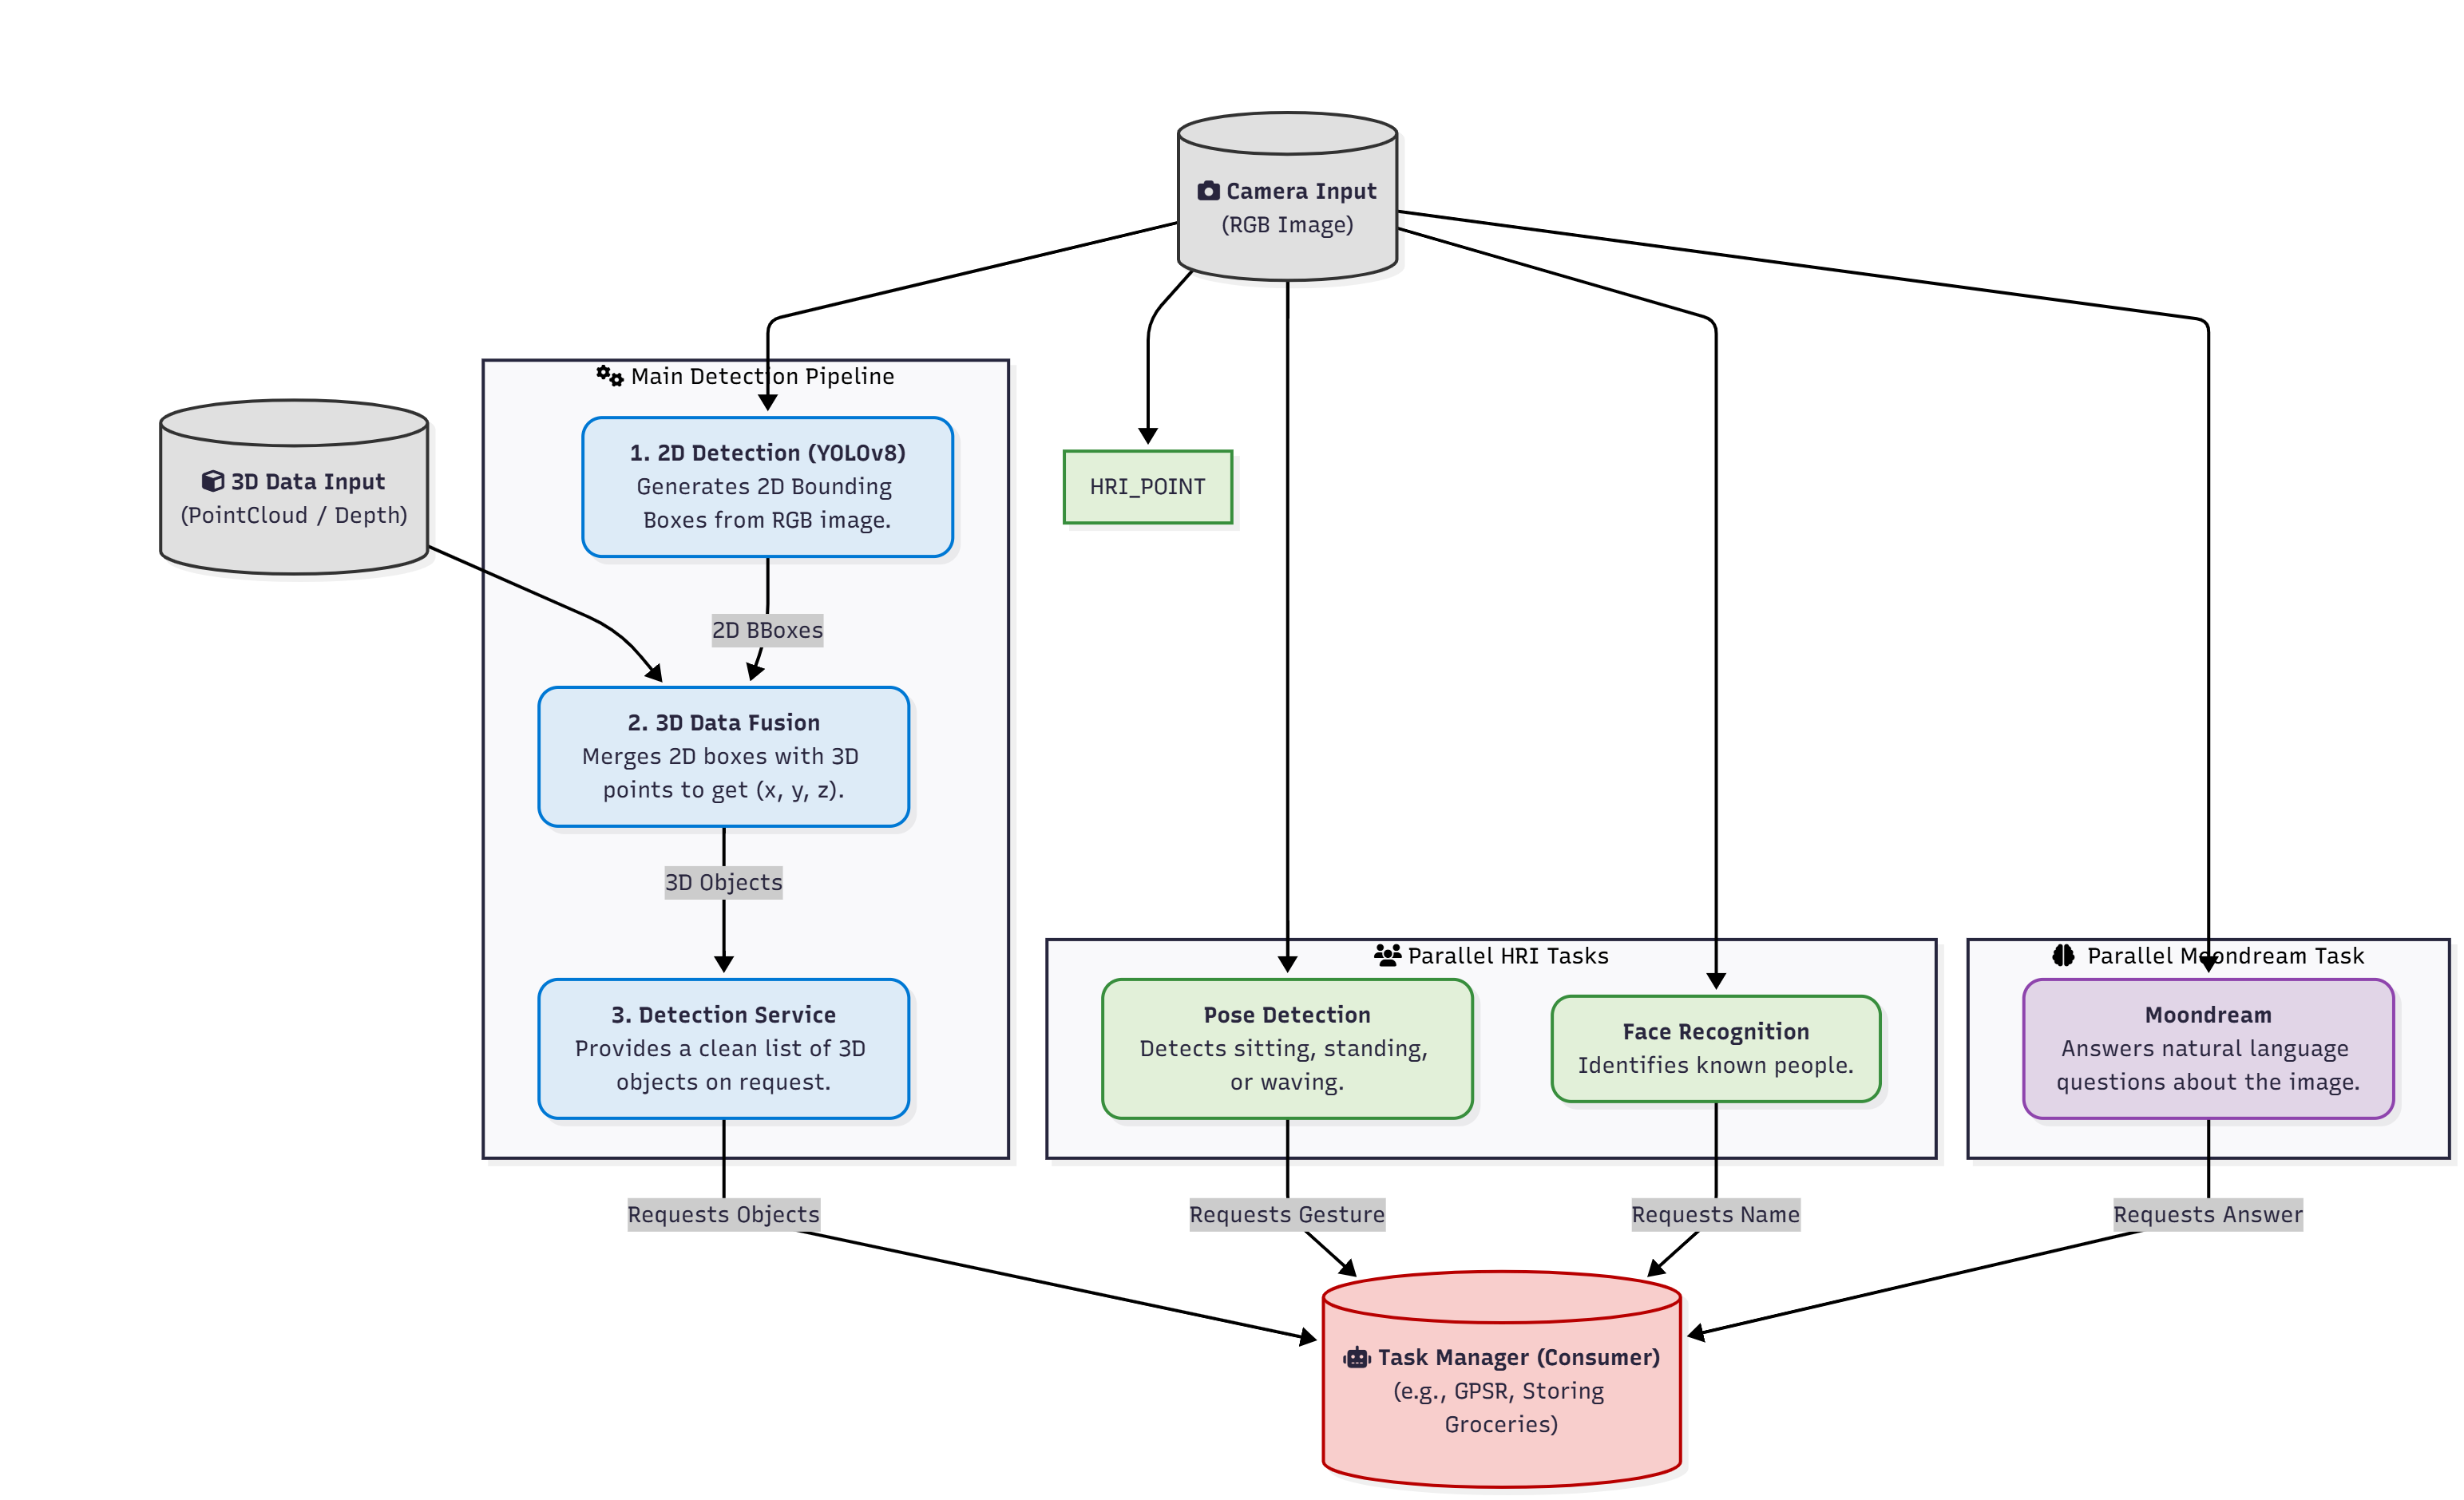
\includegraphics[width=1\textwidth]{TDPTemplate-master/images/Vision_pipeline.png}
%     \caption{Vision pipeline.}
%     \label{fig: pipeline}
% \end{figure}




% \section{HRI}

% \subsection{HRI Pipeline}
% \begin{figure}[H]
%     \centering
%     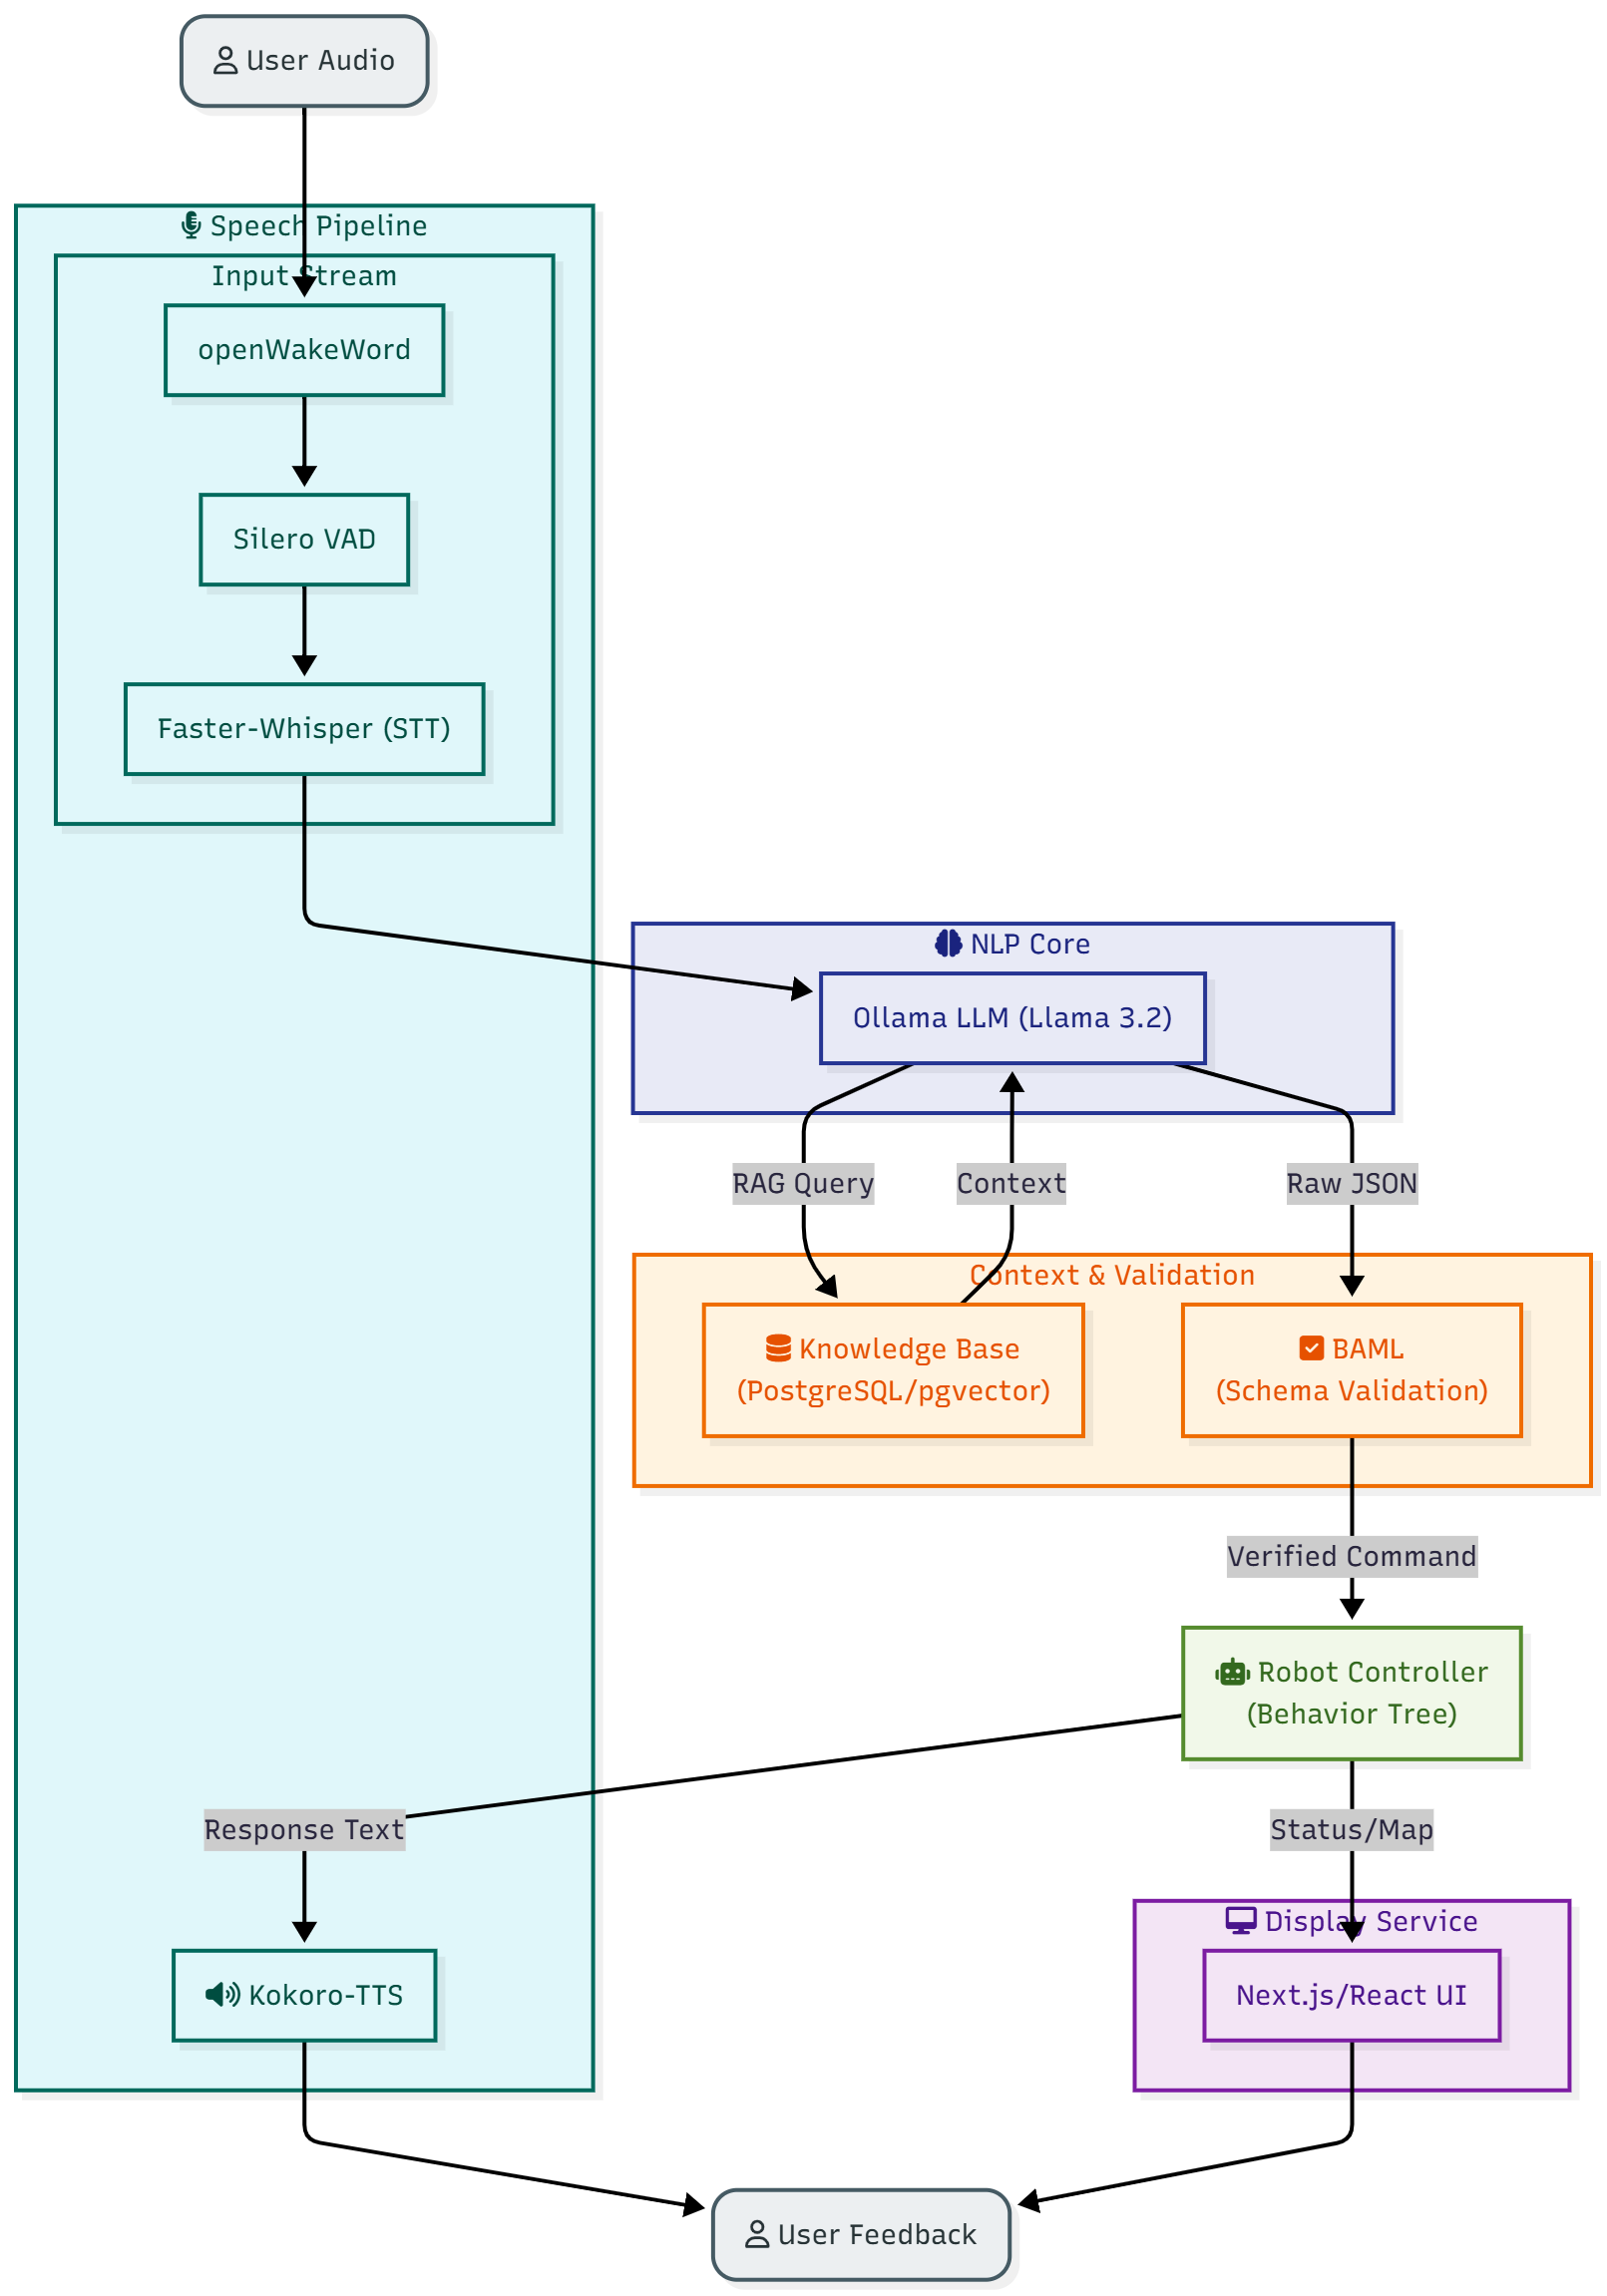
\includegraphics[width=0.6\textwidth]{TDPTemplate-master/images/HRI_pipeline.png}
%     \caption{HRI Pipeline}
%     \label{fig:hri_pipeline}
% \end{figure}

% \section{Navigation}

% \subsection{Omnibase}
% \begin{figure}[H]
%     \centering
%     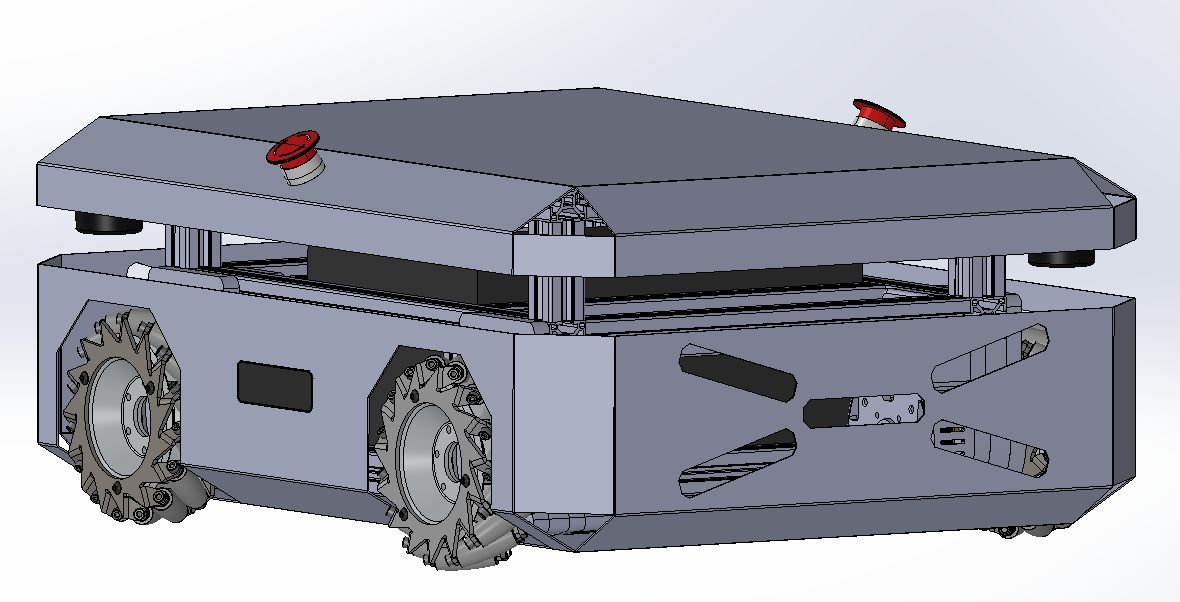
\includegraphics[width=1\textwidth]{TDPTemplate-master/images/Omnibase_CAD.jpg}
%     \caption{Omnibase CAD}
%     \label{fig:Omnibase_CAD}
% \end{figure}

% \section{Electronics}
% \subsection{PCB 3D}
% \begin{figure}[H]
%     \centering
%     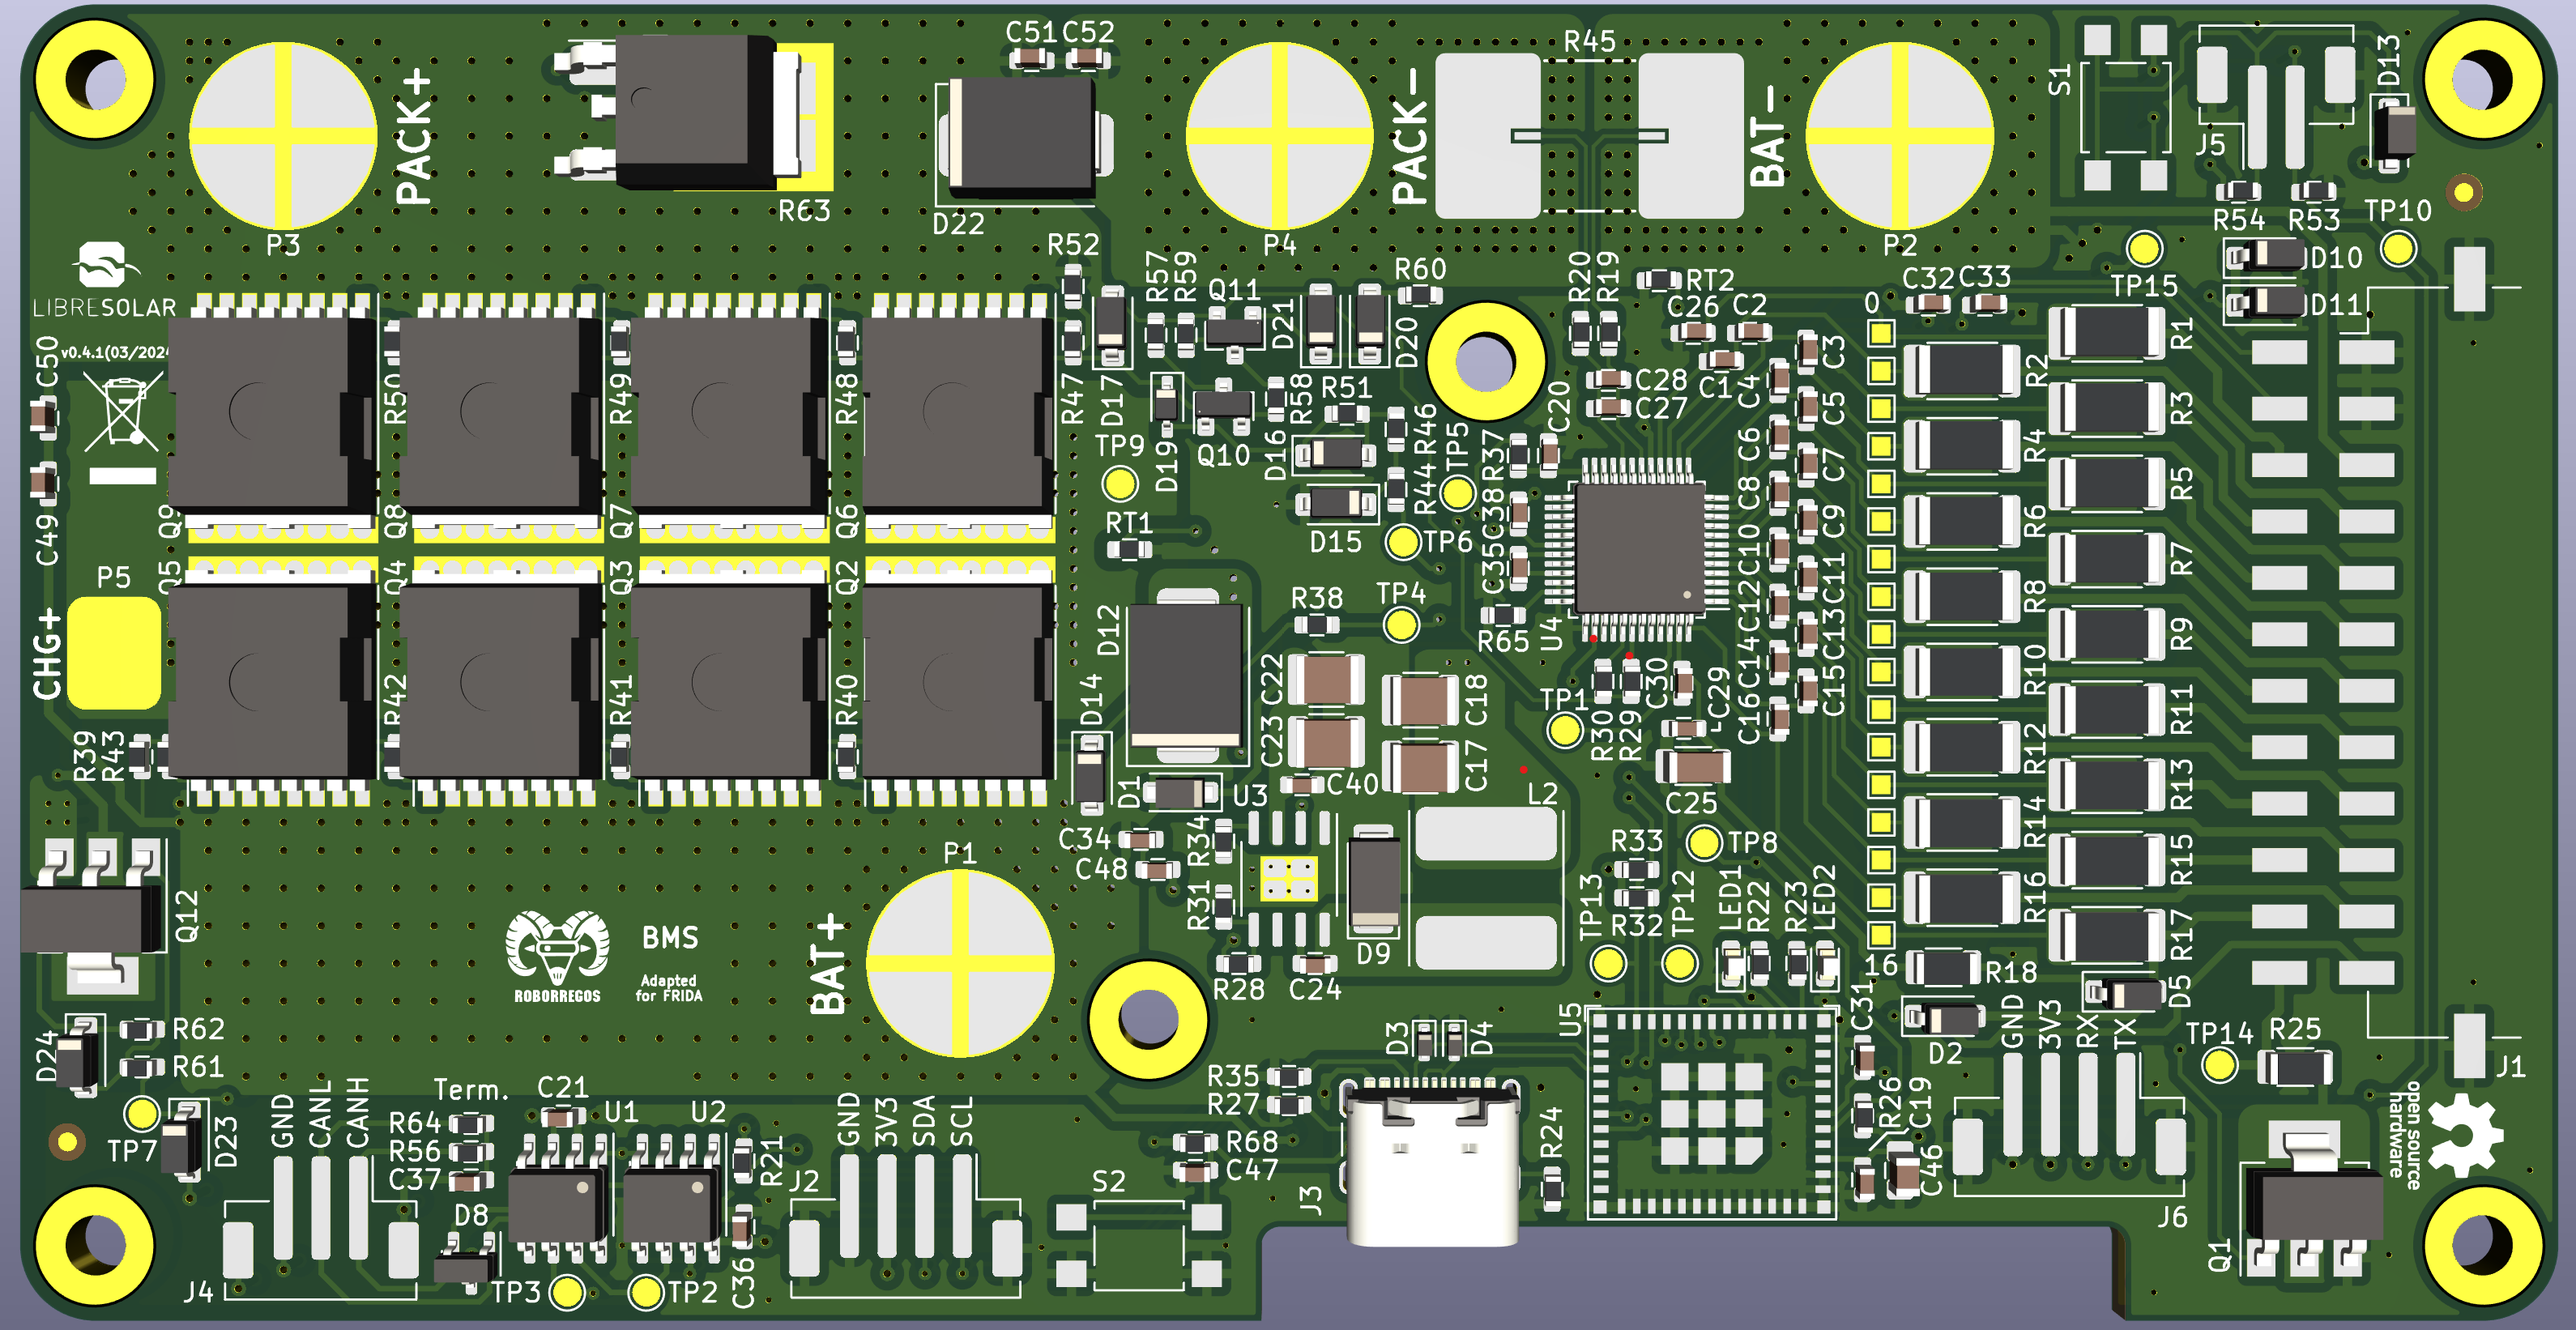
\includegraphics[width=1\textwidth]{TDPTemplate-master/images/BMS_3DView.png}
%     \caption{BMS 3D View}
%     \label{fig:BMS_3DView}
% \end{figure}

\end{document}
